\documentclass[tikz,border=12pt]{standalone}
% Match the sans-serif font stack used by the Minimal Mistakes site theme.
% TeX Gyre Heros is the TeX-compatible Helvetica implementation.
\usepackage[T1]{fontenc}
\usepackage{tgheros}
\renewcommand{\familydefault}{\sfdefault}

\usetikzlibrary{arrows.meta,positioning,fit}
\definecolor{pink}{HTML}{F06595}\definecolor{blue}{HTML}{4DABF7}\definecolor{green}{HTML}{51CF66}\definecolor{violet}{HTML}{B197FC}\definecolor{ink}{HTML}{E9ECEF}\definecolor{panel}{HTML}{211C1D}
\begin{document}
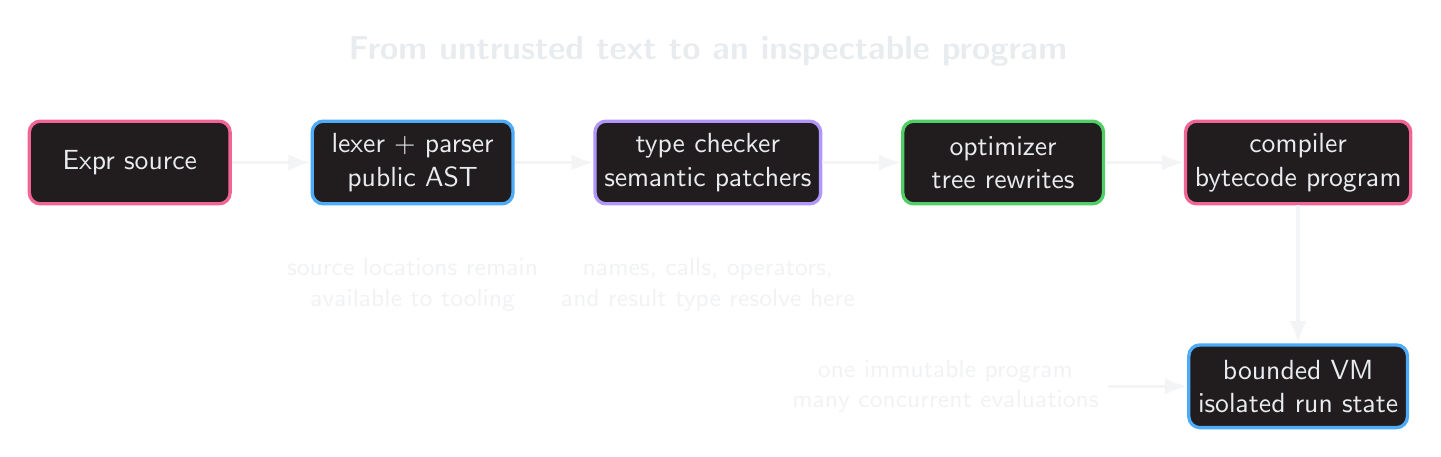
\begin{tikzpicture}[
  text=ink,
  stage/.style={rounded corners=4pt,fill=panel,very thick,minimum width=2.55cm,minimum height=1.05cm,align=center},
  arrow/.style={-{Latex[length=2.8mm]},very thick,ink!60},
  note/.style={font=\small,align=center}
]
  \node[stage,draw=pink] (source) {Expr source};
  \node[stage,draw=blue,right=1.0cm of source] (syntax) {lexer + parser\\public AST};
  \node[stage,draw=violet,right=1.0cm of syntax] (check) {type checker\\semantic patchers};
  \node[stage,draw=green,right=1.0cm of check] (opt) {optimizer\\tree rewrites};
  \node[stage,draw=pink,right=1.0cm of opt] (program) {compiler\\bytecode program};
  \node[stage,draw=blue,below=1.75cm of program] (vm) {bounded VM\\isolated run state};

  \draw[arrow] (source) -- (syntax);
  \draw[arrow] (syntax) -- (check);
  \draw[arrow] (check) -- (opt);
  \draw[arrow] (opt) -- (program);
  \draw[arrow] (program) -- (vm);

  \node[note,text=ink!70,below=.55cm of syntax] {source locations remain\\available to tooling};
  \node[note,text=ink!70,below=.55cm of check] {names, calls, operators,\\and result type resolve here};
  \node[note,text=ink!70,left=1.0cm of vm] (reuse) {one immutable program\\many concurrent evaluations};
  \draw[arrow] (reuse) -- (vm);
  \node[font=\bfseries\large,text=ink,above=.55cm of check] {From untrusted text to an inspectable program};
\end{tikzpicture}
\end{document}
